%!TEX root = ../../root.tex

How powerful is this model? Meaning, how many real functions $f$ can it represent, given the proper values for the parameters? The \emph{Stone-Weierstrass} theorem provides us with an aswer.

\begin{thm}[Stone-Weierstrass]\label{thm:stone_weiestrass}
	If $f$ is continuous on the interval $[a, b]$, then for every $\epsilon > 0$ there exists a polynomial $p$ such that $|f(x) - p(x)| < \epsilon$ for all $x$.
\end{thm}

\cref{thm:stone_weiestrass} tells us that if we are given a real function $f$ on some interval then there exists a polynomial $p$, whose degree we do not know, that \emph{globally} (i.e. for every value of its domain $x$) approximates $f$ to the desired accuracy, and the approximation is measured in the absolute error. But how to choose the degree of the polynomial? It is not a parameter to be learned, but rather an \emph{hyperparameter}, that encodes a prior we establish, e.g. we expect the data to be distributed following a cubic-like polynomial. Let's see what happens by trying to fit polynomials of various degrees to the same data.

 \begin{figure}[H]
 	\centering
	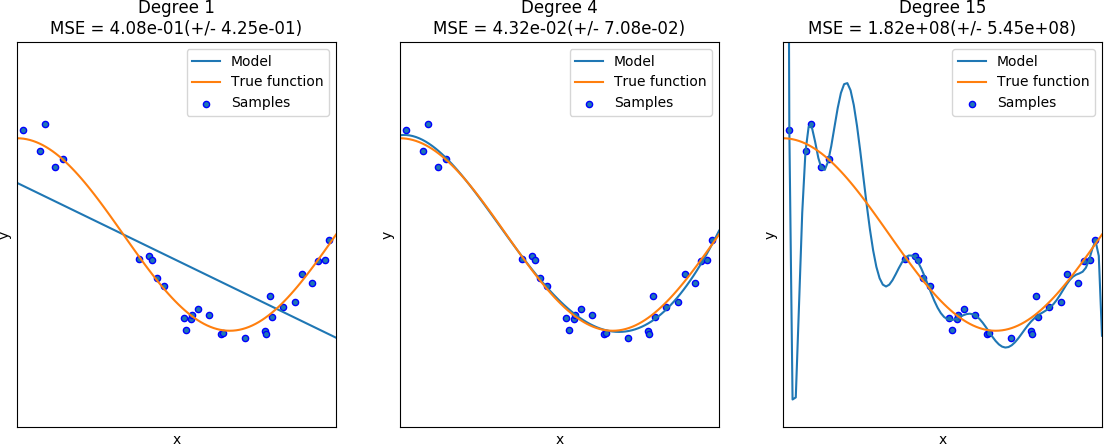
\includegraphics[width=.7\textwidth]{05/scikit3}
 	\caption{Fit data with different poly degree.}\label{fig:fit_poly}	
\end{figure}

In \cref{fig:fit_poly} we can see that with a $1$-degree polynomial we can not represent the data distribution well: we are \emph{underfitting}. With a $4$-degree polynomial we get a very good representation, so we may think that going higher we could get an even better representation.
Indeed, with a $15$-degree polynomial we get a representation that fits all points, so the \emph{MSE} for this polynomial is smaller than the $4$-degree polynomial, although we can see immediately that the representation is not something that we desire. Why is that? Because it is very unlikely that the true function that has produced these data points looks like this learned function. We are \emph{overfitting}.

These two phenomena that we observe in \cref{fig:fit_poly} are found across all deep learning, not just polynomial regression models:
\begin{itemize}
	\item \textbf{Underfitting}: not sufficiently fitting the data (large \emph{MSE}) as it happens choosing degree one polynomial;
	\item \textbf{Overfitting}: we are ``learning the noise'' as it happens choosing degree fifteen polynomial.
\end{itemize}
From the notion of overfitting we see that adding complexity to a learning model is not necessarily a good thing because it could lead to overfitting and overfitting leads to bad generalization. So there will always be a trade-off between these two phenomena.

\begin{tcolorbox}
    \textbf{Note}: Remember that we are inferring a function (an item from an infinite-dimensional space) from a finite set of training samples, therefore there necessarily will be regions of the domain not covered by the samples, in which we have no clue of the behavior of the function (this is where the priors step in). Nonetheless, we would like for the learned function to approximate the true function well overall, not only on the training data, i.e. to be as \emph{general} as possible, even if this means not fitting the training data perfectly. 
\end{tcolorbox}

There is a relatively easy way to detect whether we are doing underfitting or overfitting:
\begin{enumerate}
    \item Separate the known data into two sets: the \emph{training} set and the \emph{validation} set;
	\item Estimate the model parameters on the \emph{training} set so as to minimize the loss function on the training data;
	\item If the loss is large on the training set, then we are underfitting, since the model is not able to represent well enough the training data;
	\item If the loss is small, then we \emph{may} be overfitting. To check this, we take the \emph{validation} set and compute the loss function on these new data;
	\item If we get large loss on the validation set then we are overfitting, since the model is very good at representing the training data, but generalizes badly on unseen samples, hence the learned function cannot be a good global approximation of the true function.
\end{enumerate}
In summary, underfitting is whenever we have large training error and large validation error, while overfitting is whenever we have small training error and large validation error.

\paragraph{$k$-fold cross-validation}
There are different mechanisms that defend us from underfitting and overfitting and the simplest way that we usually employ in practice is called \emph{k-fold cross-validation}.

The key point of \emph{k-fold cross-validation} is that we do not want to overfit on the validation set either. To avoid this we split our training set in $k$ subsets which we call \emph{folds}. Then we train on $k-1$ subsets and validate on the remaining 1, and repeat this task for each subset (\textit{i.e.} $k$ times). In this way, we have the \emph{MSE} for each subset and we can take the average. If the model is getting a good score on the average over all the folds then we can say that the model is a good one, while if it does not get a good score then maybe we should change the model.
For instance, in polynomial regression we can do \emph{k-fold cross-validation} many times with different degrees and choose the run with the smallest average \emph{MSE}.

\begin{figure}[H]
	\centering
	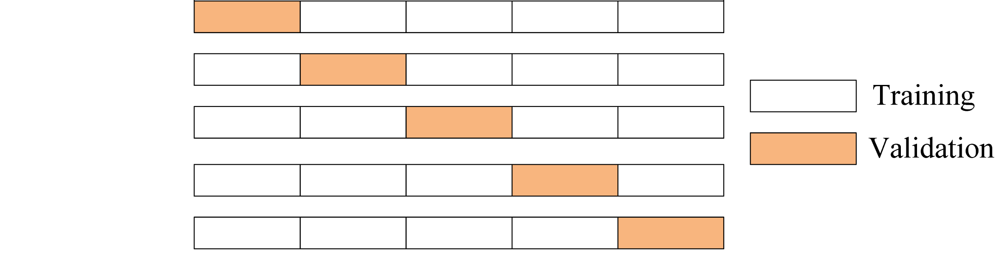
\includegraphics[width=\textwidth]{05/nfold3}
	\caption{k-fold cross validation.}\label{fig_cross_valid}	
\end{figure}

So, we said that polynomials can approximate any continuous function by \cref{thm:stone_weiestrass}, but are not enough for many reasons:
\begin{itemize}
 	\item We can have much more complicated losses which are not expressed as \emph{MSE};
 	\item Polynomial regression is not easy to regularize;
 	\item Maybe we have some other knowledge, not just training data, that we would like to inject into the model;
 	\item Some models produce intermediate features which are very helpful to address certain tasks;
 	\item Flexibility, meaning ease to access or to experiment with;
 \end{itemize} 